\documentclass[]{article}
\usepackage{lmodern}
\usepackage{amssymb,amsmath}
\usepackage{ifxetex,ifluatex}
\usepackage{fixltx2e} % provides \textsubscript
\ifnum 0\ifxetex 1\fi\ifluatex 1\fi=0 % if pdftex
  \usepackage[T1]{fontenc}
  \usepackage[utf8]{inputenc}
\else % if luatex or xelatex
  \ifxetex
    \usepackage{mathspec}
  \else
    \usepackage{fontspec}
  \fi
  \defaultfontfeatures{Ligatures=TeX,Scale=MatchLowercase}
\fi
% use upquote if available, for straight quotes in verbatim environments
\IfFileExists{upquote.sty}{\usepackage{upquote}}{}
% use microtype if available
\IfFileExists{microtype.sty}{%
\usepackage{microtype}
\UseMicrotypeSet[protrusion]{basicmath} % disable protrusion for tt fonts
}{}
\usepackage[margin=1in]{geometry}
\usepackage{hyperref}
\hypersetup{unicode=true,
            pdftitle={report},
            pdfborder={0 0 0},
            breaklinks=true}
\urlstyle{same}  % don't use monospace font for urls
\usepackage{graphicx,grffile}
\makeatletter
\def\maxwidth{\ifdim\Gin@nat@width>\linewidth\linewidth\else\Gin@nat@width\fi}
\def\maxheight{\ifdim\Gin@nat@height>\textheight\textheight\else\Gin@nat@height\fi}
\makeatother
% Scale images if necessary, so that they will not overflow the page
% margins by default, and it is still possible to overwrite the defaults
% using explicit options in \includegraphics[width, height, ...]{}
\setkeys{Gin}{width=\maxwidth,height=\maxheight,keepaspectratio}
\IfFileExists{parskip.sty}{%
\usepackage{parskip}
}{% else
\setlength{\parindent}{0pt}
\setlength{\parskip}{6pt plus 2pt minus 1pt}
}
\setlength{\emergencystretch}{3em}  % prevent overfull lines
\providecommand{\tightlist}{%
  \setlength{\itemsep}{0pt}\setlength{\parskip}{0pt}}
\setcounter{secnumdepth}{0}
% Redefines (sub)paragraphs to behave more like sections
\ifx\paragraph\undefined\else
\let\oldparagraph\paragraph
\renewcommand{\paragraph}[1]{\oldparagraph{#1}\mbox{}}
\fi
\ifx\subparagraph\undefined\else
\let\oldsubparagraph\subparagraph
\renewcommand{\subparagraph}[1]{\oldsubparagraph{#1}\mbox{}}
\fi

%%% Use protect on footnotes to avoid problems with footnotes in titles
\let\rmarkdownfootnote\footnote%
\def\footnote{\protect\rmarkdownfootnote}

%%% Change title format to be more compact
\usepackage{titling}

% Create subtitle command for use in maketitle
\providecommand{\subtitle}[1]{
  \posttitle{
    \begin{center}\large#1\end{center}
    }
}

\setlength{\droptitle}{-2em}

  \title{report}
    \pretitle{\vspace{\droptitle}\centering\huge}
  \posttitle{\par}
    \author{}
    \preauthor{}\postauthor{}
    \date{}
    \predate{}\postdate{}
  
\usepackage{booktabs}
\usepackage{longtable}
\usepackage{array}
\usepackage{multirow}
\usepackage{wrapfig}
\usepackage{float}
\usepackage{colortbl}
\usepackage{pdflscape}
\usepackage{tabu}
\usepackage{threeparttable}
\usepackage{threeparttablex}
\usepackage[normalem]{ulem}
\usepackage{makecell}
\usepackage{xcolor}

\begin{document}
\maketitle

\hypertarget{overall-performance}{%
\subsection{Overall Performance}\label{overall-performance}}

\begin{verbatim}
## Warning: Using alpha for a discrete variable is not advised.
\end{verbatim}

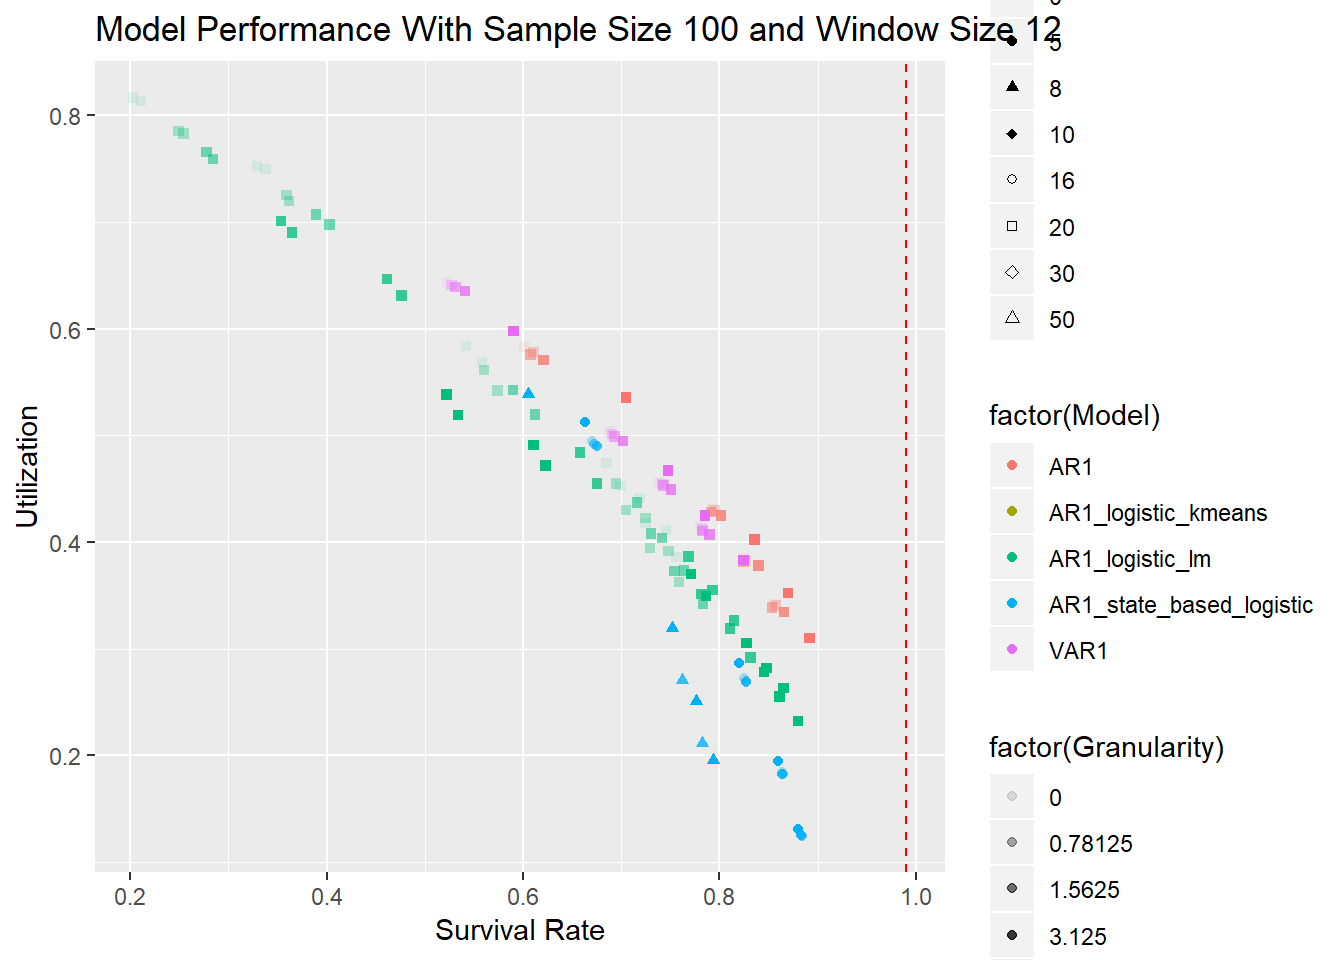
\includegraphics{report_files/figure-latex/unnamed-chunk-4-1.pdf}

\begin{verbatim}
## Warning: Using alpha for a discrete variable is not advised.
\end{verbatim}

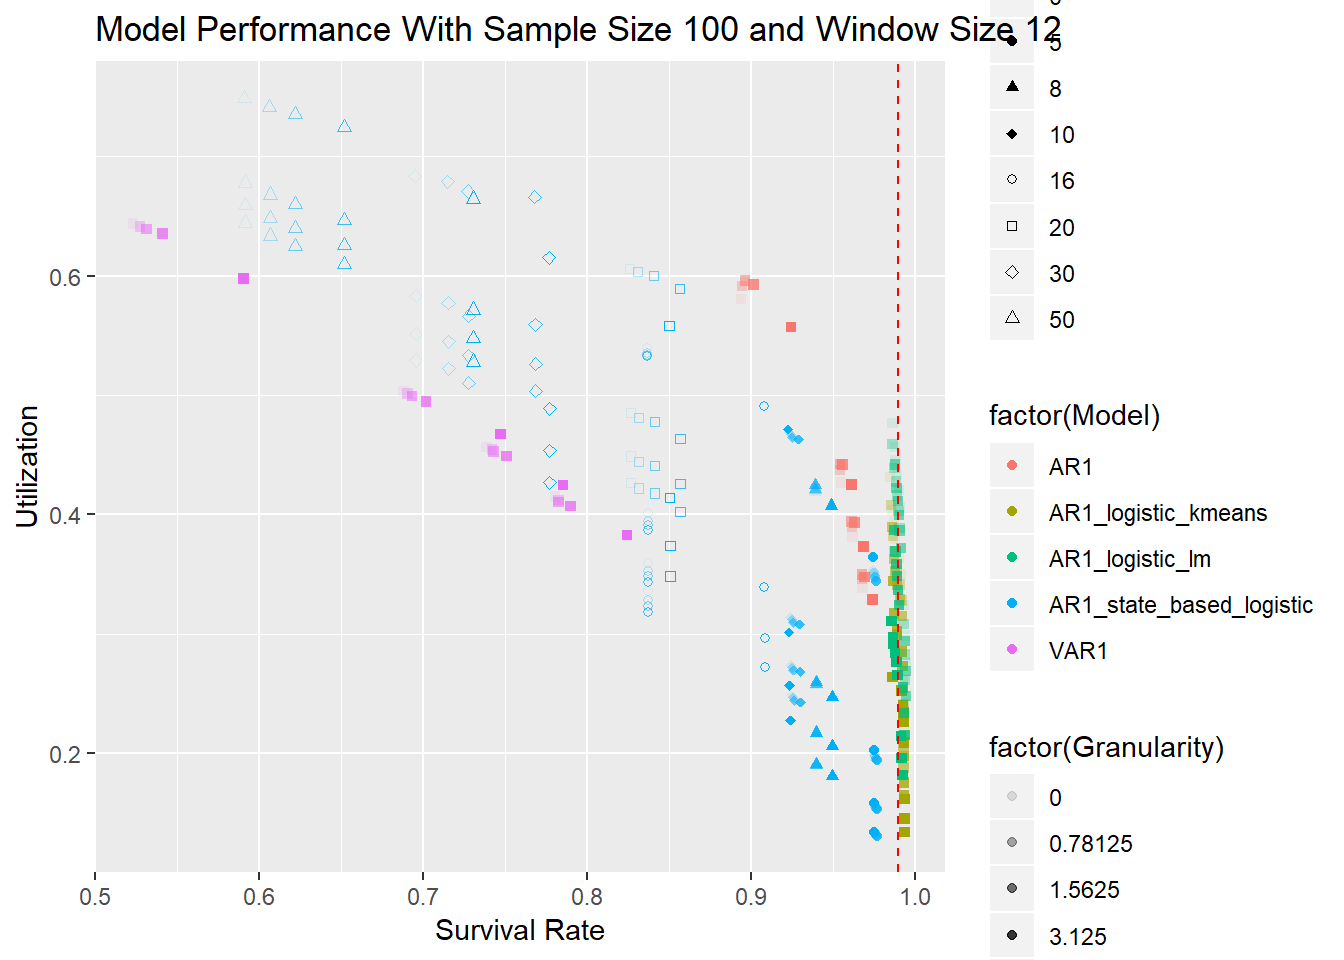
\includegraphics{report_files/figure-latex/unnamed-chunk-4-2.pdf}

\hypertarget{runs-for-different-models}{%
\subsection{Runs for Different Models}\label{runs-for-different-models}}

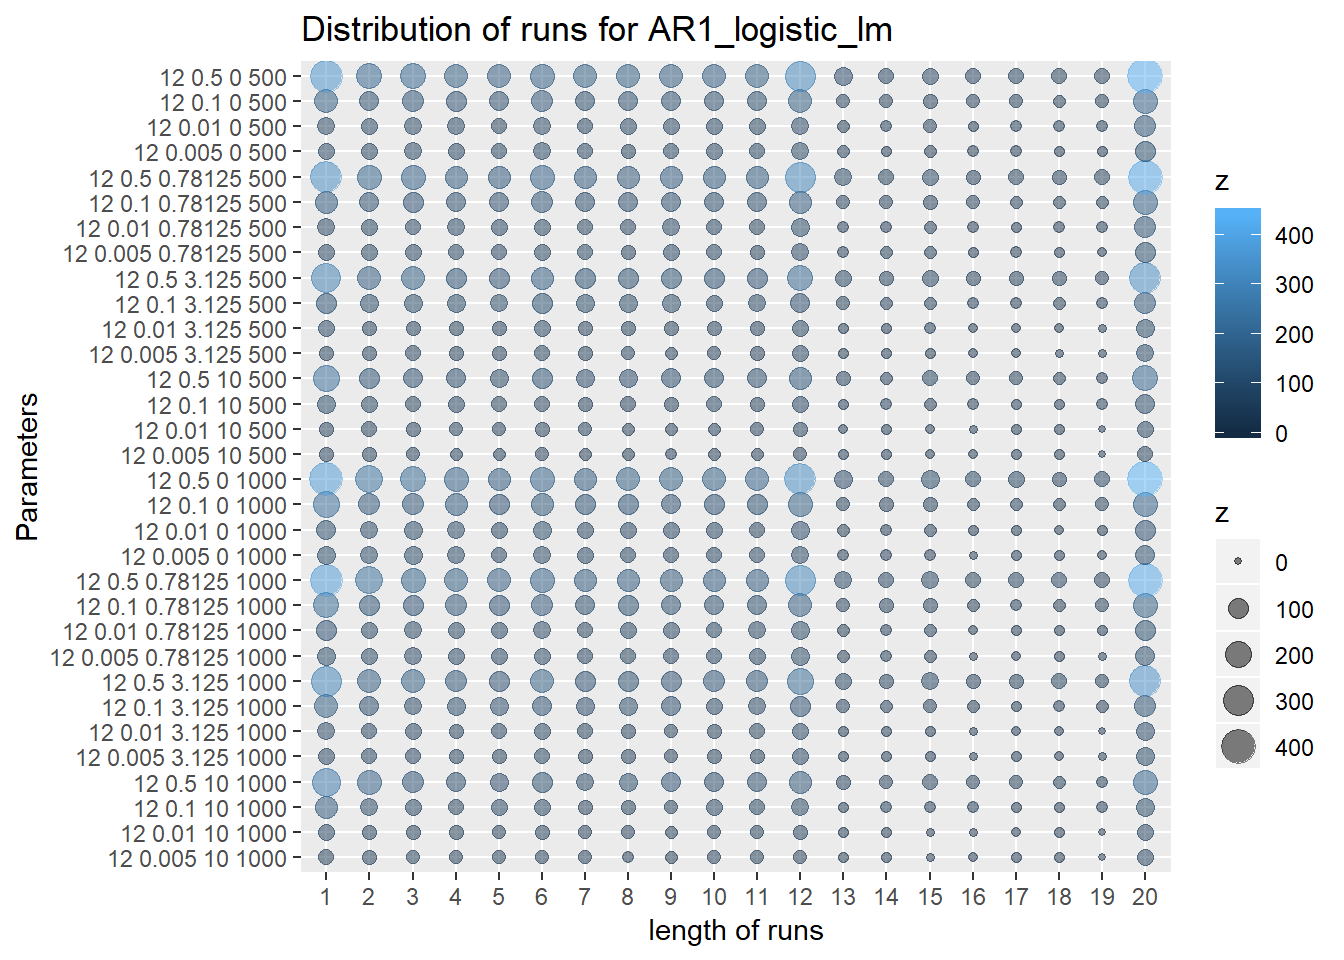
\includegraphics{report_files/figure-latex/unnamed-chunk-5-1.pdf}

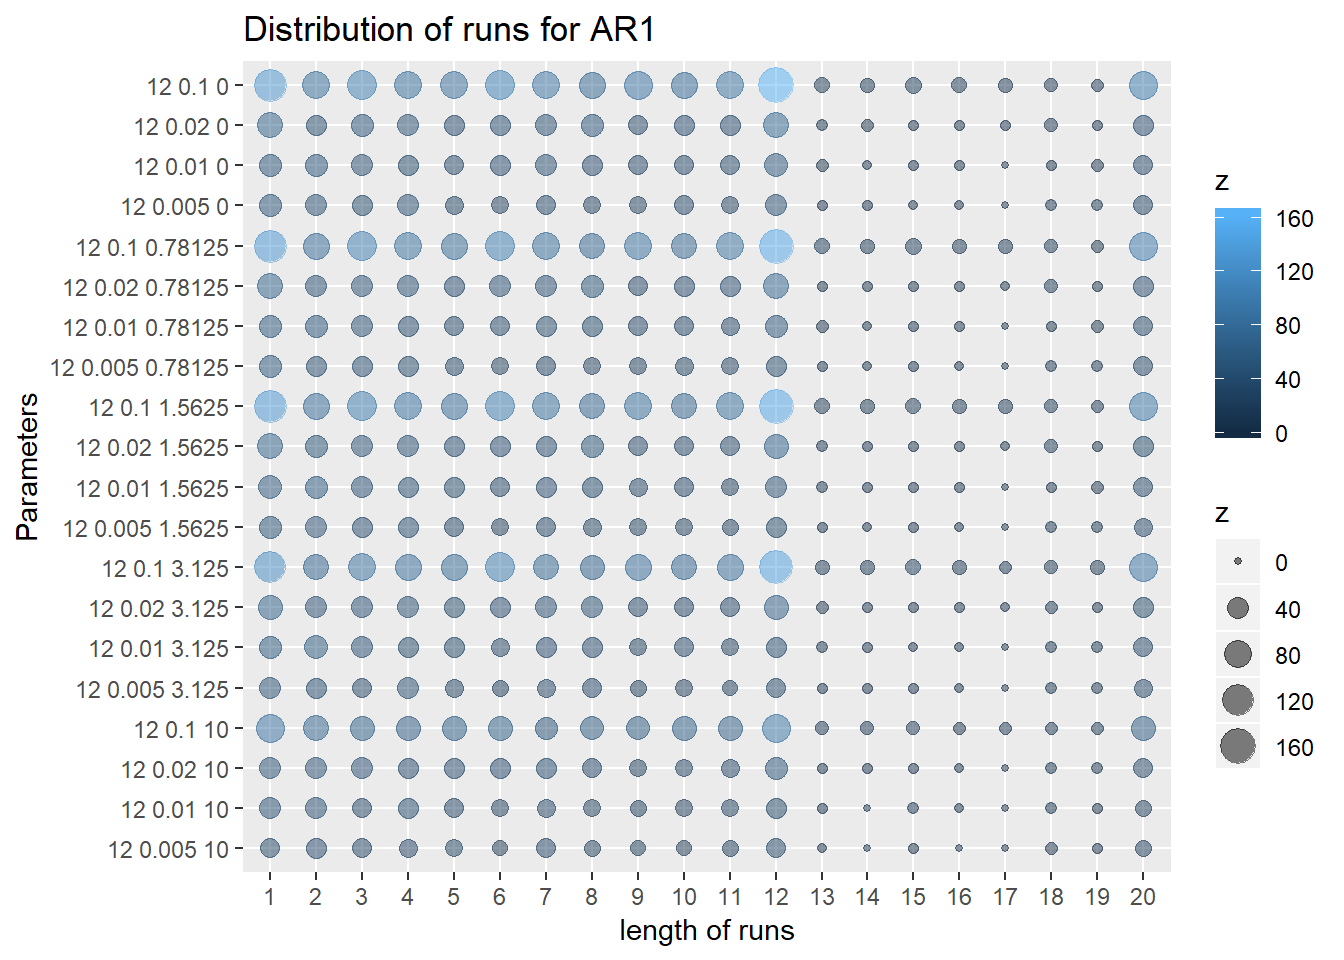
\includegraphics{report_files/figure-latex/unnamed-chunk-6-1.pdf}

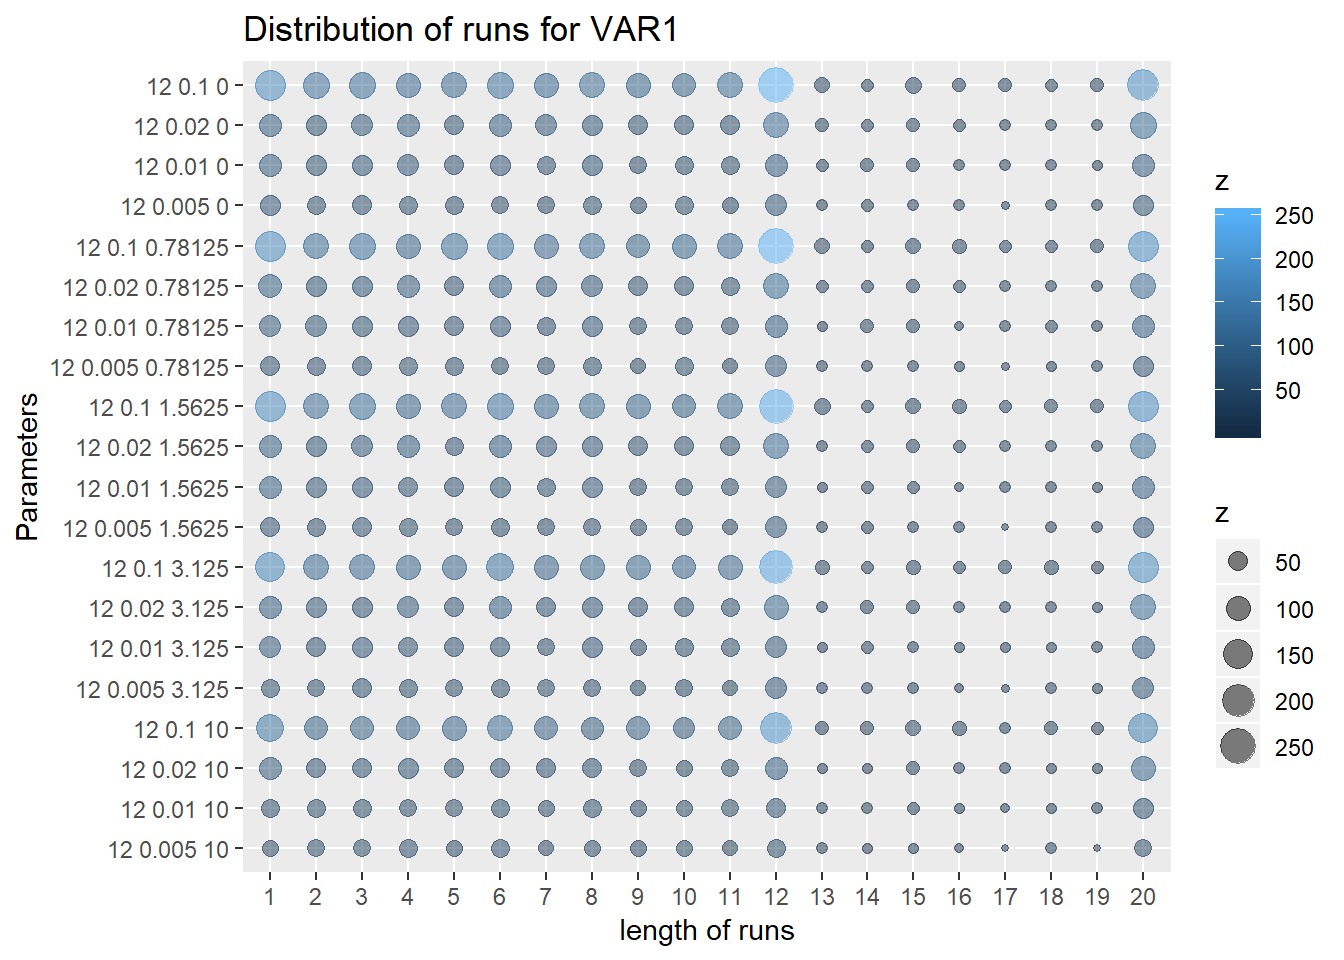
\includegraphics{report_files/figure-latex/unnamed-chunk-7-1.pdf}

\hypertarget{conditional-variance}{%
\subsection{Conditional Variance}\label{conditional-variance}}

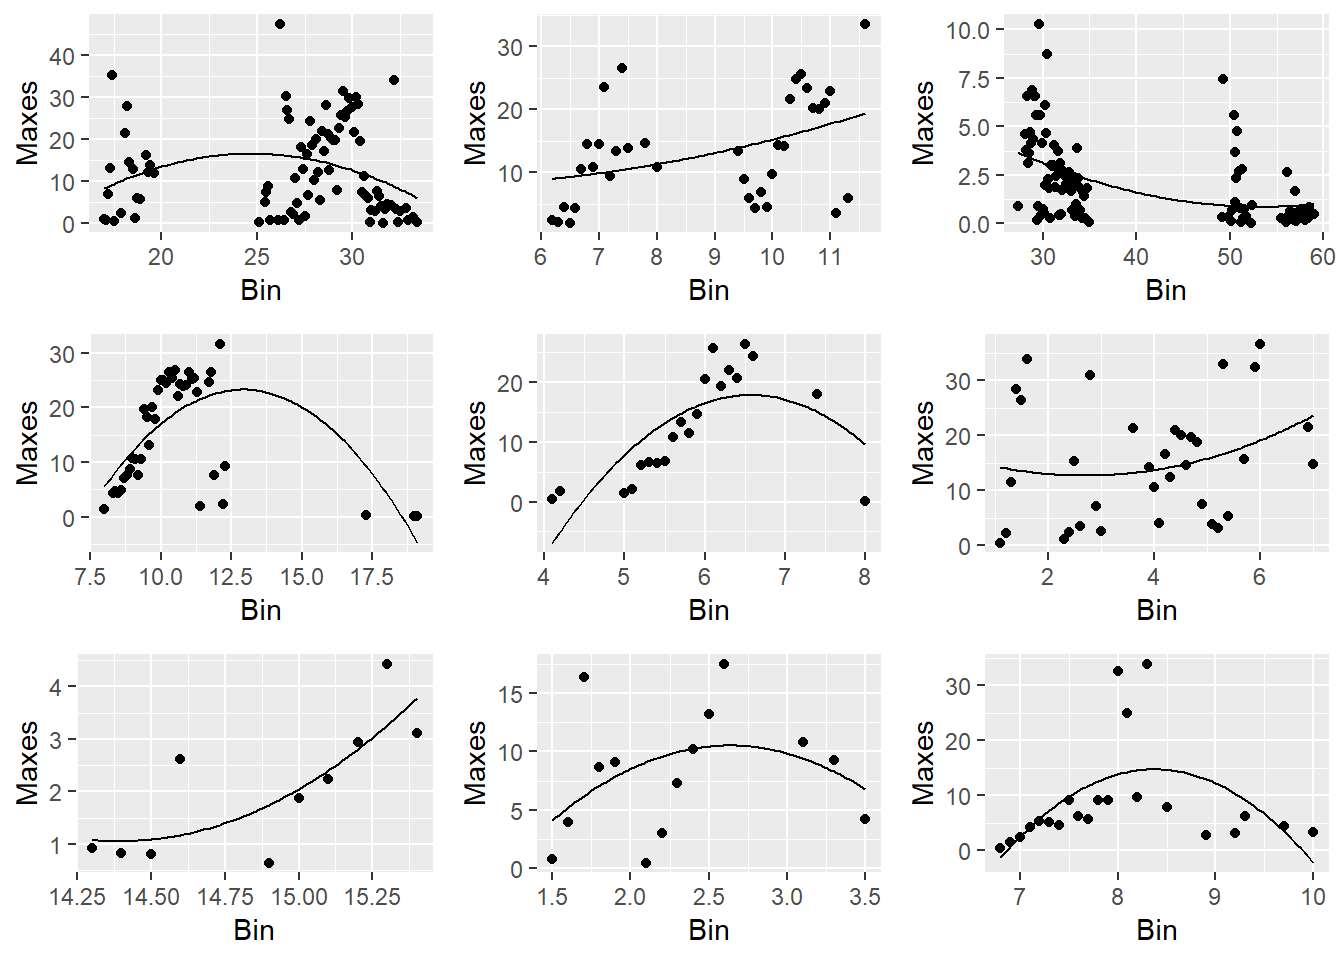
\includegraphics{report_files/figure-latex/unnamed-chunk-11-1.pdf}

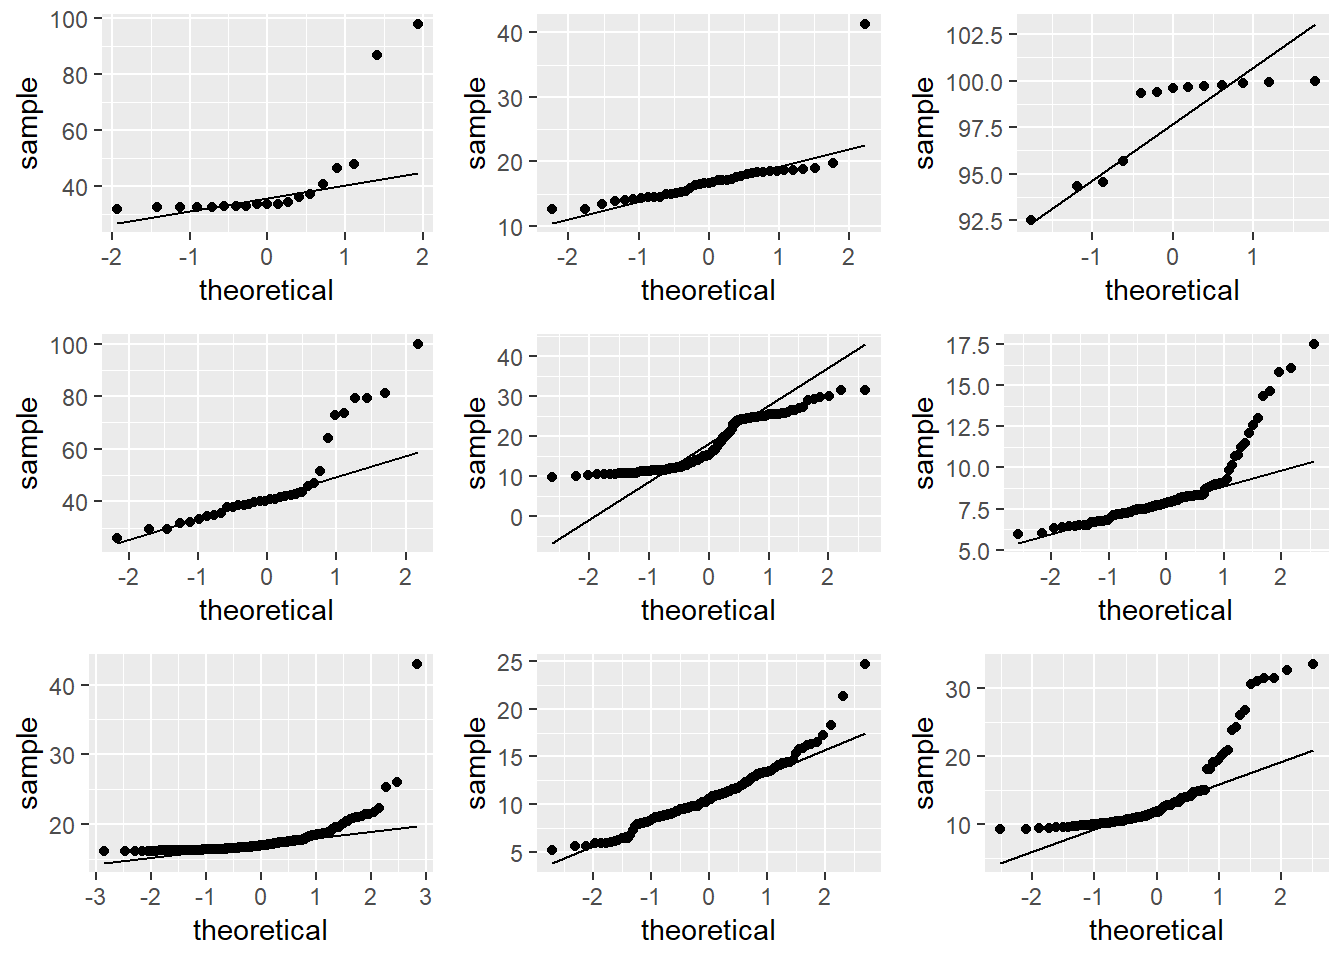
\includegraphics{report_files/figure-latex/unnamed-chunk-12-1.pdf}

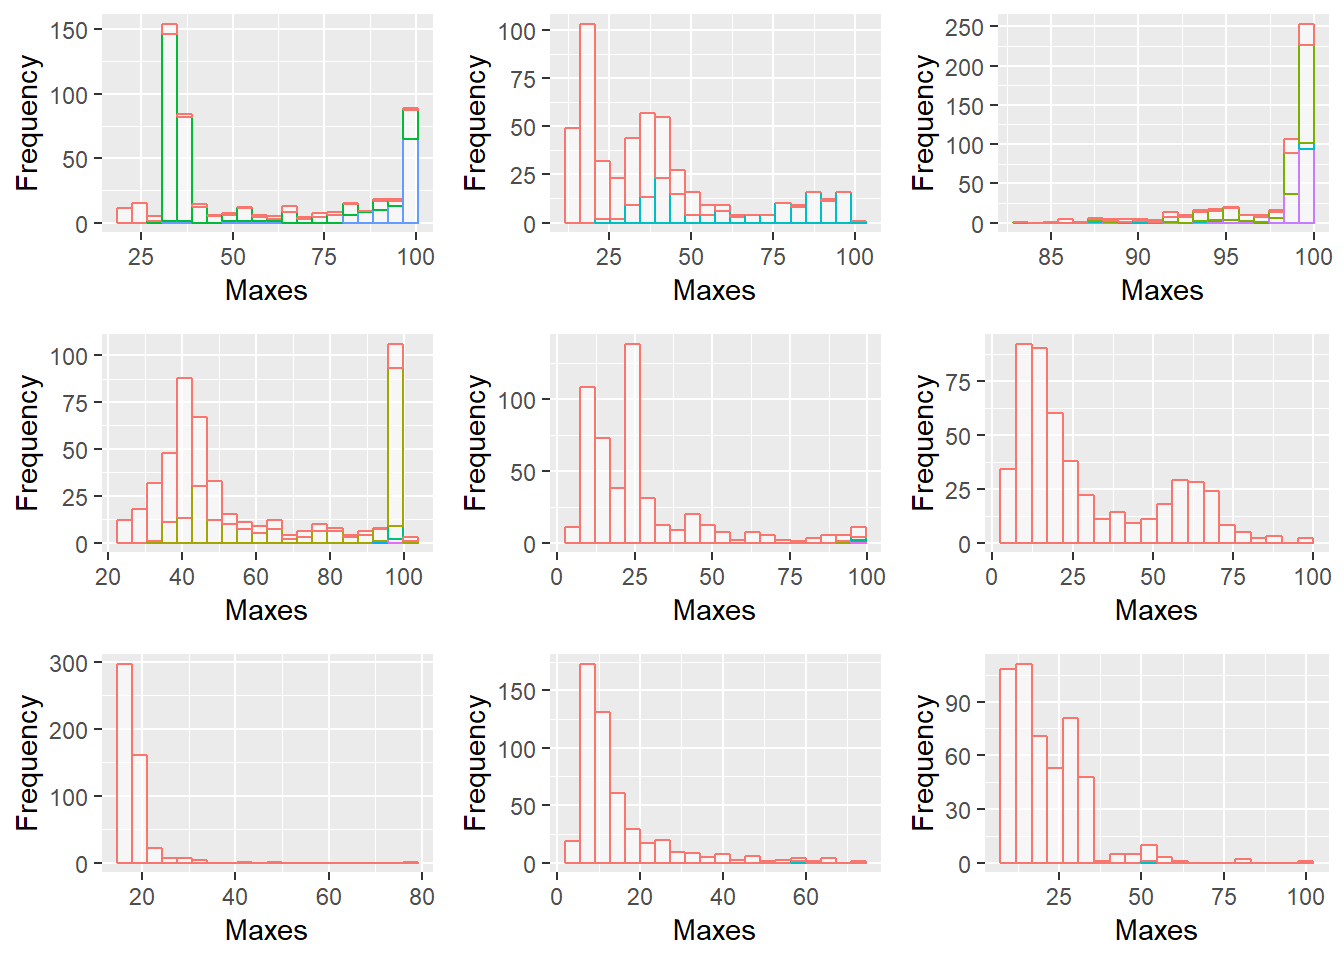
\includegraphics{report_files/figure-latex/unnamed-chunk-13-1.pdf}

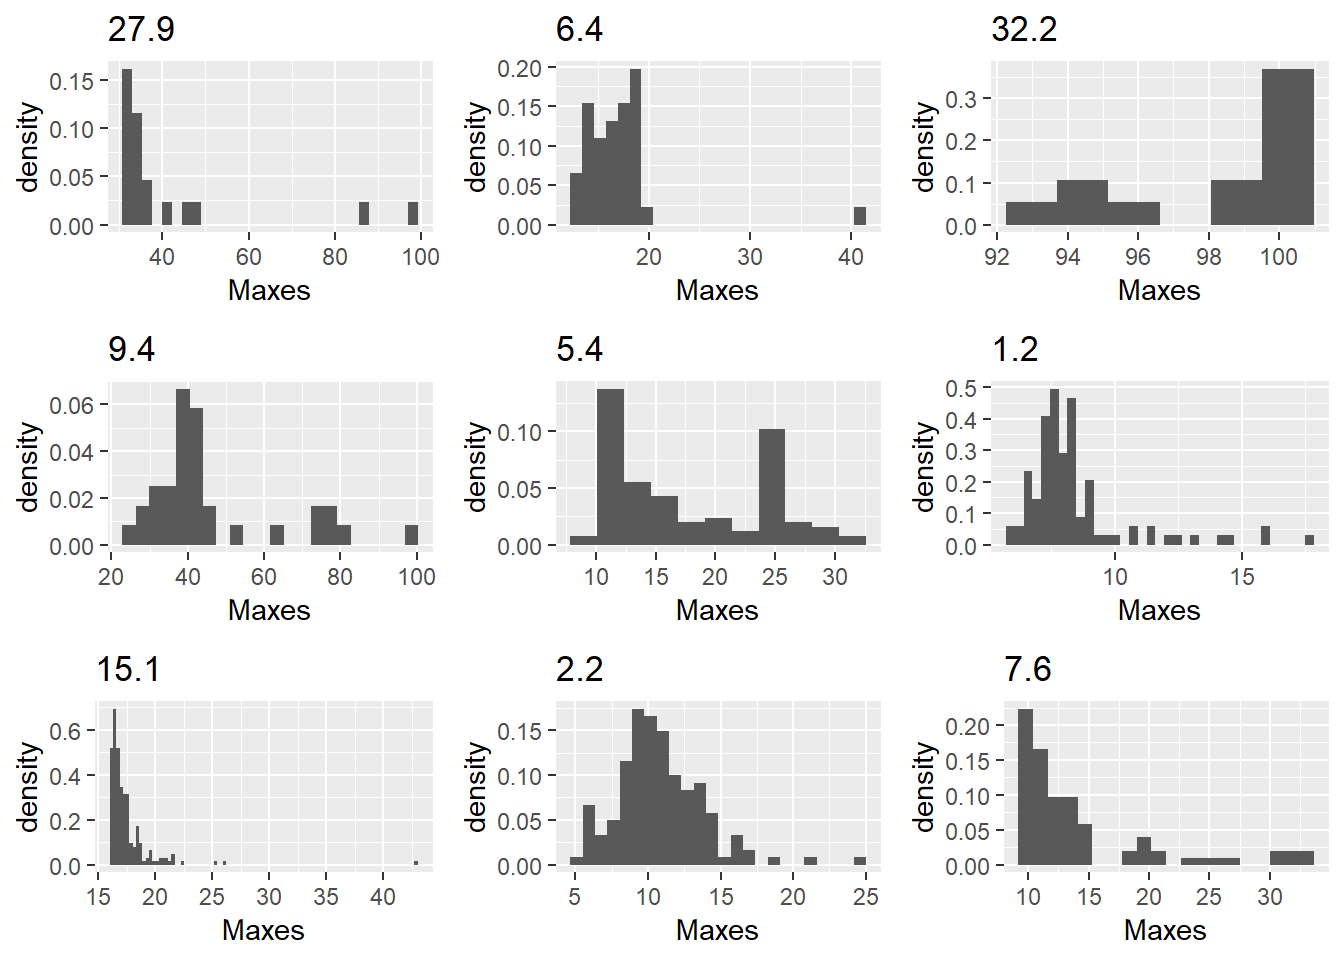
\includegraphics{report_files/figure-latex/unnamed-chunk-14-1.pdf}

\begin{verbatim}
## \begin{table}[t]
## 
## \caption{\label{tab:unnamed-chunk-15}Cut off Prob: 0.01 Granularity: 10 Bin_num: 1000}
## \centering
## \begin{tabular}{l|r|r}
## \hline
##   & avg\_usage & survival\\
## \hline
## 1633748 & 0.5172878 & 0.8913043\\
## \hline
## 8201 & 0.1967712 & 0.6470588\\
## \hline
## 827636 & 0.2319377 & 0.7083333\\
## \hline
## 965207 & 0.4342857 & 0.9880240\\
## \hline
## 948898 & 0.0015528 & 1.0000000\\
## \hline
## 1054436 & 0.0000000 & 1.0000000\\
## \hline
## 715586 & 0.5057777 & 0.7619048\\
## \hline
## 964235 & 0.0000000 & 1.0000000\\
## \hline
## 586036 & 0.0000000 & 0.9939394\\
## \hline
## \end{tabular}
## \end{table}
## \begin{table}[t]
## 
## \caption{\label{tab:unnamed-chunk-15}Cut off Prob: 0.5 Granularity: 10 Bin_num: 1000}
## \centering
## \begin{tabular}{l|r|r}
## \hline
##   & avg\_usage & survival\\
## \hline
## 1633748 & 0.8127451 & 0.4840764\\
## \hline
## 8201 & 0.7431827 & 0.2707071\\
## \hline
## 827636 & 0.5349013 & 0.3174603\\
## \hline
## 965207 & 0.5755259 & 0.9880240\\
## \hline
## 948898 & 0.0023292 & 1.0000000\\
## \hline
## 1054436 & 0.0000000 & 1.0000000\\
## \hline
## 715586 & 0.7625164 & 0.6460905\\
## \hline
## 964235 & 0.0000000 & 1.0000000\\
## \hline
## 586036 & 0.0017422 & 0.9265537\\
## \hline
## \end{tabular}
## \end{table}
## \begin{table}[t]
## 
## \caption{\label{tab:unnamed-chunk-15}Cut off Prob: 0.01 Granularity: 1.5625 Bin_num: 1000}
## \centering
## \begin{tabular}{l|r|r}
## \hline
##   & avg\_usage & survival\\
## \hline
## 1633748 & 0.5671706 & 0.8810811\\
## \hline
## 8201 & 0.2570762 & 0.4352941\\
## \hline
## 827636 & 0.2707742 & 0.7048458\\
## \hline
## 965207 & 0.7406610 & 0.8223350\\
## \hline
## 948898 & 0.3858461 & 0.9314286\\
## \hline
## 1054436 & 0.2221955 & 0.7718447\\
## \hline
## 715586 & 0.4695662 & 0.7892157\\
## \hline
## 964235 & 0.0371287 & 0.1296296\\
## \hline
## 586036 & 0.1455265 & 0.9111111\\
## \hline
## \end{tabular}
## \end{table}
## \begin{table}[t]
## 
## \caption{\label{tab:unnamed-chunk-15}Cut off Prob: 0.5 Granularity: 1.5625 Bin_num: 1000}
## \centering
## \begin{tabular}{l|r|r}
## \hline
##   & avg\_usage & survival\\
## \hline
## 1633748 & 0.9246257 & 0.2694611\\
## \hline
## 8201 & 0.7537166 & 0.2420857\\
## \hline
## 827636 & 0.5755671 & 0.2980562\\
## \hline
## 965207 & 0.9017234 & 0.4903226\\
## \hline
## 948898 & 0.7160814 & 0.5033113\\
## \hline
## 1054436 & 0.6427755 & 0.4556575\\
## \hline
## 715586 & 0.7213993 & 0.6638655\\
## \hline
## 964235 & 0.2292424 & 0.1192982\\
## \hline
## 586036 & 0.5376891 & 0.5032895\\
## \hline
## \end{tabular}
## \end{table}
## \begin{table}[t]
## 
## \caption{\label{tab:unnamed-chunk-15}Cut off Prob: 0.01 Granularity: 10 Bin_num: 500}
## \centering
## \begin{tabular}{l|r|r}
## \hline
##   & avg\_usage & survival\\
## \hline
## 1633748 & 0.5245342 & 0.8961749\\
## \hline
## 8201 & 0.1263382 & 0.7064677\\
## \hline
## 827636 & 0.1957969 & 0.7979275\\
## \hline
## 965207 & 0.0000000 & 1.0000000\\
## \hline
## 948898 & 0.0007764 & 1.0000000\\
## \hline
## 1054436 & 0.0000000 & 1.0000000\\
## \hline
## 715586 & 0.5328816 & 0.7619048\\
## \hline
## 964235 & 0.0000000 & 1.0000000\\
## \hline
## 586036 & 0.0000000 & 0.9939394\\
## \hline
## \end{tabular}
## \end{table}
## \begin{table}[t]
## 
## \caption{\label{tab:unnamed-chunk-15}Cut off Prob: 0.5 Granularity: 10 Bin_num: 500}
## \centering
## \begin{tabular}{l|r|r}
## \hline
##   & avg\_usage & survival\\
## \hline
## 1633748 & 0.8211111 & 0.4646154\\
## \hline
## 8201 & 0.7216707 & 0.2712551\\
## \hline
## 827636 & 0.5349013 & 0.3174603\\
## \hline
## 965207 & 0.2895238 & 0.9880240\\
## \hline
## 948898 & 0.0023292 & 1.0000000\\
## \hline
## 1054436 & 0.0000000 & 1.0000000\\
## \hline
## 715586 & 0.8006729 & 0.4228571\\
## \hline
## 964235 & 0.0000000 & 1.0000000\\
## \hline
## 586036 & 0.0017422 & 0.9939394\\
## \hline
## \end{tabular}
## \end{table}
## \begin{table}[t]
## 
## \caption{\label{tab:unnamed-chunk-15}Cut off Prob: 0.01 Granularity: 1.5625 Bin_num: 500}
## \centering
## \begin{tabular}{l|r|r}
## \hline
##   & avg\_usage & survival\\
## \hline
## 1633748 & 0.5757658 & 0.8265306\\
## \hline
## 8201 & 0.1777906 & 0.5597015\\
## \hline
## 827636 & 0.2461130 & 0.7048458\\
## \hline
## 965207 & 0.5175601 & 0.9880240\\
## \hline
## 948898 & 0.2834723 & 0.9314286\\
## \hline
## 1054436 & 0.2240410 & 0.7395349\\
## \hline
## 715586 & 0.4552828 & 0.7892157\\
## \hline
## 964235 & 0.0375000 & 0.1332487\\
## \hline
## 586036 & 0.0710382 & 0.9111111\\
## \hline
## \end{tabular}
## \end{table}
## \begin{table}[t]
## 
## \caption{\label{tab:unnamed-chunk-15}Cut off Prob: 0.5 Granularity: 1.5625 Bin_num: 500}
## \centering
## \begin{tabular}{l|r|r}
## \hline
##   & avg\_usage & survival\\
## \hline
## 1633748 & 0.9288432 & 0.2311828\\
## \hline
## 8201 & 0.7391376 & 0.2425373\\
## \hline
## 827636 & 0.5796295 & 0.3075221\\
## \hline
## 965207 & 0.7864031 & 0.7740385\\
## \hline
## 948898 & 0.6751527 & 0.5500000\\
## \hline
## 1054436 & 0.6421536 & 0.4542683\\
## \hline
## 715586 & 0.7852121 & 0.6305221\\
## \hline
## 964235 & 0.1726871 & 0.1192982\\
## \hline
## 586036 & 0.5099308 & 0.5496454\\
## \hline
## \end{tabular}
## \end{table}
\end{verbatim}


\end{document}
